In diesem Kapitel soll die generelle Funktionsweise eine Voice Assistants anhand eines Schaubilds dargestellt werden. Anschließend wird auf die einzelnen Bestandteile kurz eingegangen.

\begin{figure}[htb]
	\centering
	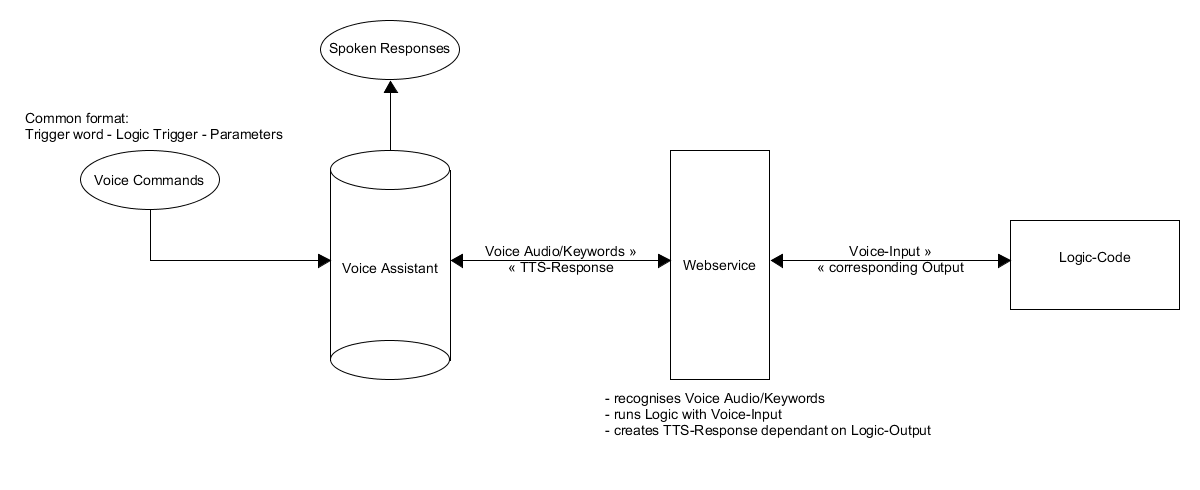
\includegraphics[scale=0.36]{content/img/GeneralVA_Architektur.png}
	\caption{Komponentendiagramm der generellen Funktionsweise eines Voice Assistants}
	\label{imgDiagramm}
\end{figure}

Wie in Abbildung \ref{imgDiagramm} beschrieben ist, muss der VA zunächst durch ein Trigger word aktiviert werden. Darauf folgt die so genannte Utterance. Diese setzt sich aus Logic Trigger und gegebenenfalls notwendigen Parametern zusammen. Diese wird mithilfe von SE auf dem Gerät erkannt und digitalisiert. Anschließend sendet der VA die Utterance an einen Webservice, der die weitere Verarbeitung übernimmt. So können die Voice Assistants schlank gehalten werden, da ein Großteil der Rechenarbeit auf dem Webservice erfolgt. \newline

Der Webservice erkennt nun anhand des Logic Triggers den konkreten Anwendungsfall und ermittelt, falls nötig, die gegebenen Parameter. Der konkrete Anwendungsfall wird als Intent bezeichnet. Die Anfrage wird daraufhin vom Webservice bearbeitet. Hierzu wird der auf einem Webserver abgelegten Logic-Code verwendet. Für jeden definierten Intent enthält der Logic-Code eine passende Funktion. Dies kann von einer einfachen Rechnung, über Suchanfragen im Internet bis hin zur Wiedergabe von akustischen Medien auf dem VA reichen.\newline

Der Logic-Code generiert eine zur Anfrage passenden Antwort, welche an den Webservice weitergereicht wird. Der Webservice erzeugt daraus eine TTS-Response, welche an den Voice Assistant gesendet wird. Letzterer ist nun in der Lage dem Anwender eine gesprochene Antwort auf seine Anfrage zu geben.